\documentclass[10pt,a4paper]{article}
% for margining standards
\usepackage[left=3cm,right=3cm,top=3cm,bottom=3cm]{geometry}
% for counting references as a section
\usepackage[numbib,notlof,notlot,nottoc]{tocbibind}
% useful packages
\usepackage{
                graphicx, setspace, fontspec, caption,
                subcaption, float, polyglossia, rotating,
                lscape, pdflscape, indentfirst, tocloft,
                multirow, mathtools, currfile
            }
% paragraph related package
\usepackage[parfill]{parskip}
% use bzar font(THIS MUST BE LOADED BEFORE XePerian PACKAGE)
\setmainfont{BZar.ttf}
% the dear XePersian package
\usepackage{xepersian}
%
% General settings goes here.
%
% lines space
\renewcommand{\baselinestretch}{1.5}
% paragraph first line indention
\setlength{\parindent}{1cm}
% paragraph spacing
\setlength{\parskip}{1em}
% set graphics' path
\graphicspath{ {images/} }
% make table of content dotted
\renewcommand{\cftsecleader}{\cftdotfill{\cftdotsep}}
% define a new command as {half-space} in english
\newcommand{\halfspace}{\hspace{0pt}}
% define a new command as {half-space} in persian
\newcommand{\نیمفاصله}{\halfspace}
% define a shortcut for half-space in general
\renewcommand{\ }{\halfspace}
% define a new command for ease of use for rendering reference
\newcommand{\renderref}[1] { \begingroup \let\clearpage\relax \include{#1} \endgroup }
% define shortcut for \mu_{\bar{A}}
\newcommand{\mba}{\mu_{\bar{A}}}
% define shortcut for \mu_{\bar{B}}
\newcommand{\mbb}{\mu_{\bar{B}}}
%
% DOCUMENT BEGIN
%
\begin{document}
\title{
    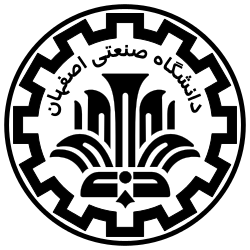
\includegraphics[width=0.25\textwidth]{iut}\\\vspace{30pt}
    بدست آوردن عملگرهای بدون پارامتری\\
    \lr{drastic} ، \lr{min} و \lr{max}\\
    از عمگلرهای پارامتری\\
    \lr{Hamcher} ، \lr{Yager} و \lr{Dubois}
}
\author{داریوش حسن\ پور آده}
\date{۹۳۰۸۱۶۴}
\maketitle
\null
\vfill
% make this very first page un-numbered
\thispagestyle{empty}
\setcounter{page}{0}
\newpage
\قسمت{مقدمه}
در این تمرین هدف  بدست آوردن عملگرهای بدون پارامتری
\lr{drastic} ، \lr{min} و \lr{max}
از عمگلرهای پارامتری
\lr{Hamcher} ، \lr{Yager} و \lr{Dubois}
که در قسمت\ های زیر به ترتیب روند بدست آوردن آنها آورده شده است.
\tableofcontents
\newpage
\قسمت{معرفی اوپراتورهای پارامتری}
روابط اوپراتورهای پارامتری به صورت جدول
\ref{tab:parametric}
می\ باشند.
\begin{table}[H]
    \centering
    \begin{latin}
    \let\oldarraystretch\arraystretch
    \renewcommand{\arraystretch}{5}
    \vspace{-2em}
        \begin{tabular}{ ll }
            Hamacher &$\begin{cases}
            Intersection:&
            \mu_{\bar{A}\cap\bar{B}}(x) = \frac{\mba(x)\mbb(x)}{\gamma + (1-\gamma)(\mba(x) + \mbb(x) - \mba(x)\mbb(x))}\\\\
            Union:& \mu_{\bar{A}\cup\bar{B}}(x) = \frac{(\gamma^\prime - 1)\mba(x)\mbb(x) + \mba(x) + \mbb(x)}{1+\gamma^\prime\mba(x)\mbb(x)}
            \end{cases}$\\
            Yager &$\begin{cases}
            Intersection:& \mu_{\bar{A}\cap\bar{B}}(x) = 1 - \min\{1, ((1-\mba(x))^p + (1-\mbb(x))^p)^{\frac{1}{p}}\},\hspace{10pt} p \geq 1\\\\
            Union:& \mu_{\bar{A}\cup\bar{B}}(x) = min\{1, (\mba(x)^p + \mbb(x)^p) ^ {\frac{1}{p}}\},\hspace{10pt} p \geq 1
            \end{cases}$\\
            Dubois &$\begin{cases}
            Intersection:& \mu_{\bar{A}\cap\bar{B}}(x) = \frac{\mba(x).\mbb(x)}{\max\{\mba(x), \mbb(x), \alpha\}}\\\\
            Union:& \mu_{\bar{A}\cup\bar{B}}(x) = \frac{\mba(x) + \mbb(x) - \mba(x).\mbb(x) - \min\{\mba(x), \mu_{\bar{B}(x)}, (1-\alpha)\}}{\max\{(1-\mba(x)), (1-\mbb(x)), \alpha\}}
            \end{cases}$
        \end{tabular}
        \let\arraystretch\oldarraystretch
    \end{latin}
    \caption{روابط معادلات پارامتری}
    \label{tab:parametric}
\end{table} 
\قسمت{اوپراتور دراستیک}
\زیرقسمت{توسط اوپراتور هماچر}
\زیرزیرقسمت{اوپراتور ضرب دراستیک}
برای بدست آوردن اوپراتور ضرب دراستیک\زیرنویس{\lr{drastic}} باید در اوپراتور اشتراکی هماچر\زیرنویس{\lr{Hamacher}} مقدار $\gamma$ را به سمت بی\ نهایت سوق دهیم؛ یعنی:
\begin{equation}
\lim_{\gamma \rightarrow \infty} \frac{\mba(x)\mbb(x)}{\gamma + (1-\gamma)(\mba(x) + \mbb(x) - \mba(x)\mbb(x))}
\label{eq:ham-int}
\end{equation}
برای حل حد
\ref{eq:ham-int}
می\ توانیم دو فرض داشته باشیم اول اینکه در مخرج شرط
\ref{cond:ham-int}
 حاکم باشد؛ آنگاه حد
\ref{eq:ham-int}
را می\ توان به صورت حد
\ref{eq:ham-int-res1}
بازنویسی کرد.
\begin{equation}
\max\{\mba(x),\mbb(x)\} \neq 1 \Longrightarrow 0 < \overbrace{\mba(x) + \mbb(x) - \mba(x)\mbb(x)} ^ \beta < 1
\label{cond:ham-int}
\end{equation}
\begin{equation}
\lim_{\gamma \rightarrow \infty} \frac{\mba(x)\mbb(x)}{\gamma + (1-\gamma)\beta} = 
\lim_{\gamma \rightarrow \infty} \frac{\mba(x)\mbb(x)}{\beta + (1 - \beta)\gamma} = 0 
\label{eq:ham-int-res1}
\end{equation}
حال اگر حداقل یکی از مقادیر
$\mba(x)$ و $\mbb(x)$
حداکثر -- یعنی برابر با ۱ شود آنگاه حد
\ref{eq:ham-int}
به صورت حد
\ref{eq:ham-int-res2}
می\ شود.
\begin{equation}
\lim_{\gamma \rightarrow \infty} \frac{\mba(x)\mbb(x)}{\gamma + (1-\gamma)} = \mba(x)\mbb(x)
\xrightarrow{\max\{\mba(x),\mbb(x)\} = 1} \min\{\mba(x),\mbb(x)\}
\label{eq:ham-int-res2}
\end{equation}
که از روابط
\ref{cond:ham-int}\ldots\ref{eq:ham-int-res2}
نتیجه\ ی
\ref{eq:ham-int-res-total}
می\ گیریم که همان معادل با
\lr{Drastic Product}
می\ باشد.
\begin{equation}\footnotesize
\lim_{\gamma \rightarrow \infty} \frac{\mba(x)\mbb(x)}{\gamma + (1-\gamma)(\mba(x) + \mbb(x) - \mba(x)\mbb(x))} = \begin{cases}
\min\{\mba(x),\mbb(x)\} & if \max\{\mba(x),\mbb(x)\} = 1\\
0 & otherwise
\end{cases}
\label{eq:ham-int-res-total}
\end{equation}
\زیرزیرقسمت{اوپراتور جمع دراستیک}
برای بدست آوردن اوپراتور جمع دراستیک باید در اوپراتور اجتماع هماچر مقدار $\gamma ^ \prime$ را به سمت منفی\ بی\ نهایت سوق دهیم؛ یعنی:
\begin{equation}
\lim_{\gamma^\prime \rightarrow -\infty} \frac{(\gamma^\prime - 1)\mba(x)\mbb(x) + \mba(x) + \mbb(x)}{1+\gamma^\prime\mba(x)\mbb(x)}
\label{eq:ham-un}
\end{equation}
در حد
\ref{eq:ham-un}
اگر حداقل یکی از مقادیر
$\mba(x)$ و $\mbb(x)$
حداقل -- یعنی برابر با ۰ شوند آنگاه حد
\ref{eq:ham-un}
به حد
\ref{eq:ham-un-res1}
تبدیل می\ شود.
\begin{equation}
\lim_{\gamma^\prime \rightarrow -\infty} \frac{\mba(x) + \mbb(x)}{1} = \mba(x) + \mbb(x) \xrightarrow{\min\{\mba(x),\mbb(x)\} = 0} \max\{\mba(x),\mbb(x)\}
\label{eq:ham-un-res1}
\end{equation}
و اگر در حد
\ref{eq:ham-un}
شرط
$\min\{\mba(x),\mbb(x)\} > 0$
برقرار باشد، طبق قضیه\ ی حدی هوپیتال، مقدار حد برابر با ۱ می\ شود. پس با توجه به روابط
\ref{eq:ham-un} و \ref{eq:ham-un-res1}
می\ توان اوپراتور جمع دراستیک را همانطور که رابطه\ ی
\ref{eq:ham-un-total}
نشان می\ دهد بدست آورد.
\begin{equation}\small
\lim_{\gamma^\prime \rightarrow -\infty} \frac{(\gamma^\prime - 1)\mba(x)\mbb(x) + \mba(x) + \mbb(x)}{1+\gamma^\prime\mba(x)\mbb(x)} = \begin{cases}
\max\{\mba(x),\mbb(x)\} & if \min\{\mba(x),\mbb(x)\} = 0\\
1 & otherwise
\end{cases}
\label{eq:ham-un-total}
\end{equation}
\زیرقسمت{توسط اوپراتور یاگر}
\زیرزیرقسمت{اوپراتور ضرب دراستیک}
برای بدست آوردن اوپراتور ضرب دراستیک باید در اوپراتور اشتراک یاگر\زیرنویس{\lr{Yager}} مقدار $p$ را به سمت ۰ سوق دهیم؛ یعنی:
\begin{equation}
\lim_{p \rightarrow 0} 1 - \min\{1, ((1-\mba(x))^p + (1-\mbb(x))^p)^{\frac{1}{p}}\}
\label{eq:yag-int}
\end{equation}
در حد
\ref{eq:yag-int}
در صورتی که فرض
\ref{eq:yag-int-cond}
را داشته باشیم آنگاه به جواب حدی
\ref{eq:yag-int-part1}
می\ رسیم.
\begin{equation}
\max\{\mba(x), \mbb(x)\} = 1
\label{eq:yag-int-cond}
\end{equation}
\begin{equation}
\begin{split}
    \max\{\mba(x), \mbb(x)\} = 1 \xRightarrow{Assume\hspace{5pt}\mba(x) = 1} \lim_{p \rightarrow 0} 1 - \min\{1, (0^p + (1-\mbb(x))^p)^{\frac{1}{p}}\}\\
    = 1 - \min\{1, 1 - \mbb(x)\} = \mbb(x)\hspace{10pt}
\end{split}
\label{eq:yag-int-part1}
\end{equation}
و رابطه\ ی
\ref{eq:yag-int-part1}
را می\ توان برای
${\footnotesize \mbb(x) = 1}$
نیز نوشت و در نهایت می\ توان نتیجه\ ی
\ref{eq:yag-int-part2}
را گرفت.
\vspace{1.4em}\begin{equation}\footnotesize
\max\{\mba(x), \mbb(x)\} = 1 \Longrightarrow \lim_{p \rightarrow 0} 1 - \min\{1, ((1-\mba(x))^p + (1-\mbb(x))^p)^{\frac{1}{p}}\} = \min\{\mba(x) , \mbb(x)\}
\label{eq:yag-int-part2}\vspace{1em}
\end{equation}
حال در صورتی که فرض
\ref{eq:yag-int-cond}
را نداشته باشیم، آنگاه بدون اینکه به کلیت مساله لطمه\ ای وارد شود می\ توانیم فرض
\ref{eq:yag-int-part3}
کنیم.
\begin{equation}
\mba(x) > \mbb(x) \Longrightarrow (1 - \mba(x)) < (1 - \mbb(x)) 
\label{eq:yag-int-part3}
\end{equation}
با توجه به فرض
\ref{eq:yag-int-part3}
حد
\ref{eq:yag-int}
را می\ توان به صورت زیر بازنویسی کرد.
\begin{equation}
\begin{split}
\lim_{p \rightarrow 0} 1 - \min\{1, ((1-\mba(x))^p + (1-\mbb(x))^p)^{\frac{1}{p}}\}\hspace{5em}\\
= \lim_{p \rightarrow 0} 1 - \min\{1, [(1-\mba(x))^p(1 + (\frac{1-\mbb(x)}{1-\mba(x)})^p]^{\frac{1}{p}}\}\\
= \lim_{p \rightarrow 0} 1 - \min\{1, (1-\mba(x))[1 + (\frac{1-\mbb(x)}{1-\mba(x)})^p]^{\frac{1}{p}}\}\\
\xRightarrow{|\frac{1-\mbb(x)}{1-\mba(x)}| > 1} 1 - \min\{1, \infty\} = 0
\end{split}
\label{eq:yag-int-part4}
\end{equation}
که مشابه شرط
\ref{eq:yag-int-part3}
 و اثبات حدی
\ref{eq:yag-int-part4}
می\ توان برای
$\mbb(x)$
نیز نوشت
که از روابط
\ref{eq:yag-int}\ldots\ref{eq:yag-int-part4}
نتیجه\ ی
\ref{eq:yag-int-total}
را می\ گیریم که همان معادل با
\lr{Drastic Product}
می\ باشد.
\begin{equation}\footnotesize
\lim_{p \rightarrow 1} 1 - \min\{1, ((1-\mba(x))^p + (1-\mbb(x))^p)^{\frac{1}{p}}\} = \begin{cases}
\min\{\mba(x) , \mbb(x)\} & if \max\{\mba(x) , \mbb(x)\} = 1\\
0 & otherwise
\end{cases}
\label{eq:yag-int-total}
\end{equation}
\زیرزیرقسمت{اوپراتور جمع دراستیک}
برای بدست آوردن اوپراتور جمع دراستیک باید که در اوپراتور اجتماع یاگر مقدار $p$ را به سمت ۰ سوق دهیم؛ یعنی:
\begin{equation}
\lim_{p \rightarrow 0} min\{1, (\mba(x)^p + \mbb(x)^p) ^ {\frac{1}{p}}\}
\label{eq:yag-un}
\end{equation}
در حد
\ref{eq:yag-un}
در صورتی که فرض
\ref{eq:yag-un-cond}
را داشته باشیم آنگاه به جواب حدی
\ref{eq:yag-un-part1}
می\ رسیم.
\begin{equation}
\min\{\mba(x), \mbb(x)\} = 0
\label{eq:yag-un-cond}
\end{equation}
\begin{equation}
\begin{split}
    \min\{\mba(x), \mbb(x)\} = 0 \xRightarrow{Assume\hspace{5pt}\mba(x) = 0} \lim_{p \rightarrow 0} \min\{1, (0^p + \mbb(x)^p)^{\frac{1}{p}}\}\\
    = \min\{1, \mbb(x)\} = \mbb(x)\hspace{1pt}
\end{split}
\label{eq:yag-un-part1}
\end{equation}
و رابطه\ ی
\ref{eq:yag-un-part1}
را می\ توان برای
${\footnotesize \mbb(x) = 0}$
نوشت و در نهایت می\ توان نتیجه\ ی
\ref{eq:yag-un-part2}
را گرفت.
\begin{equation}
\min\{\mba(x), \mbb(x)\} = 0 \Longrightarrow \lim_{p \rightarrow 0} min\{1, (\mba(x)^p + \mbb(x)^p) ^ {\frac{1}{p}}\} = \max\{\mba(x) , \mbb(x)\}
\label{eq:yag-un-part2}
\end{equation}
حال در صورتی که فرض
\ref{eq:yag-un-cond}
را نداشته باشیم آنگاه با توجه به سوق $p \rightarrow 0$ مقدار
\ref{eq:yag-un-part3}
را داریم.
\begin{equation}
(\mba(x)^p + \mbb(x)^p)^{\frac{1}{p}} \gg 1
\label{eq:yag-un-part3}
\end{equation}
که با توجه به مقدار
\ref{eq:yag-un-part3}
جواب حدی
\ref{eq:yag-un}
به صورت
\ref{eq:yag-un-part4}
می\ شود.
\begin{equation}
\lim_{p \rightarrow 0} \min\{1, (\mba(x)^p + \mbb(x)^p)^{\frac{1}{p}}\} = 1
\label{eq:yag-un-part4}
\end{equation}
که از روابط
\ref{eq:yag-un}\ldots\ref{eq:yag-un-part4}
نتیجه\ ی
\ref{eq:yag-un-total}
را می\ گیریم که همان معادل با
\lr{Drastic Sum}
می\ باشد.
\begin{equation}
\lim_{p \rightarrow 1} min\{1, (\mba(x)^p + \mbb(x))^p) ^ {\frac{1}{p}}\} = \begin{cases}
\max\{\mba(x) , \mbb(x)\} & if \min\{\mba(x) , \mbb(x)\} = 0\\
1 & otherwise
\end{cases}
\label{eq:yag-un-total}
\end{equation}
\قسمت{اوپراتور $min$}
\زیرقسمت{توسط اوپراتور یاگر}
برای بدست آوردن اوپراتور مینیمم\زیرنویس{\lr{Minimum}} باید در اوپراتور اشتراک یاگر مقدار $p$ را به سمت بی\ نهایت سوق دهیم؛ یعنی:
\begin{equation}
\lim_{p \rightarrow \infty} 1 - \min\{1, ((1-\mba(x))^p + (1-\mbb(x))^p)^{\frac{1}{p}}\}
\label{eq:min-yag-int}
\end{equation}
حال اگه فرض 
\ref{eq:yag-int-cond}
را داشته باشیم همان نتایج
\ref{eq:yag-int-part1} و \ref{eq:yag-int-part2}
 را داریم. و اگر فرض 
\ref{eq:yag-int-cond}
را نداشته باشیم آنگاه با توجه به
$p \rightarrow \infty$
مقدار زیر را داریم. طبق قضایای حدی و بدون اینکه به کلیت مساله لطمه\ ای وارد شود فرض
$(1 - \mba(x)) > (1 - \mbb(x)) \Longleftarrow \mba(x) < \mbb(x)$
را می\ کنیم و در نتیجه جواب حدی
\ref{eq:min-yag-part1}
را داریم.
\begin{equation}
\begin{split}
\lim_{p \rightarrow \infty} 1 - \min\{1, ((1-\mba(x))^p + (1-\mbb(x))^p)^{\frac{1}{p}}\}\hspace{5.5em}\\
= \lim_{p \rightarrow \infty} 1 - \min\{1, [(1-\mba(x))^p(1 + (\frac{1-\mbb(x)}{1-\mba(x)})^p)]^{\frac{1}{p}}\}\\
= \lim_{p \rightarrow \infty} 1 - \min\{1, (1-\mba(x))[1 + (\frac{1-\mbb(x)}{1-\mba(x)})^p]^{\frac{1}{p}}\}\hspace{4pt}\\
\xRightarrow{|\frac{1-\mbb(x)}{1-\mba(x)}| < 1} 1 - \min\{1, (1-\mba(x))\} = 1 - (1-\mba(x)) = \mba(x)
\end{split}
\label{eq:min-yag-part1}
\end{equation}
حدگیری رابطه\ ی
\ref{eq:min-yag-part1}
را نیز می\ توان با فرض
$(1 - \mba(x)) < (1 - \mbb(x)) \Longleftarrow \mba(x) > \mbb(x)$
نیز نوشت که در حالت کلی جواب حد
\ref{eq:min-yag-int}
به صورت
\ref{eq:min-yag-int-total}
می\ باشد که همان اوپراتور
\lr{minimum}
می\ باشد.
\begin{equation}
\lim_{p \rightarrow \infty} 1 - \min\{1, ((1-\mba(x))^p + (1-\mbb(x))^p)^{\frac{1}{p}}\} = \min\{\mba(x), \mbb(x)\}
\label{eq:min-yag-int-total}
\end{equation}
\زیرقسمت{توسط اوپراتور دوبیس}
برای بدست آوردن اوپراتور مینیمم باید در اوپراتور اشتراک دوبیس\زیرنویس{\lr{Dubois}} مقدار $\alpha$ را به سمت 0 سوق دهیم؛ یعنی:
\begin{equation}
\lim_{\alpha \rightarrow 0} \frac{\mba(x).\mbb(x)}{\max\{\mba(x), \mbb(x), \alpha\}}
\label{eq:min-dub}
\end{equation}
با توجه به تعریف ۳-۱۷ کتاب\
\cite{ZIM}
رابطه\ ی
\ref{eq:min-dub-part1}
را داریم.
\begin{equation}
\mu_{\bar{A} \cap \bar{B}}(x) = \min\{\mba(x), \mbb(x)\}\hspace{3em}for\hspace{5pt}\mba(x), \mbb(x) \in [\alpha, 1]
\label{eq:min-dub-part1}
\end{equation}
حال در صورتی که در رابطه\ ی
\ref{eq:min-dub-part1}
مقدار $\alpha$ را به سمت ۰ سوق دهیم و همچنین می دانیم که
\[0 \leq \mba(x) , \mbb(x) \leq 1\]
جواب حدی
\ref{eq:min-dub}
برابر با مقدار رابطه\ ی
\ref{eq:min-dub-part1}
می\ شود.
\قسمت{اوپراتور $max$}
\زیرقسمت{توسط اوپراتور یاگر}
برای بدست آوردن اوپراتور ماکسیمم\زیرنویس{\lr{Maximum}} باید در اوپراتور اجتماع یاگر مقدار $p$ را به سمت بی\ نهایت سوق دهیم؛ یعنی:
\begin{equation}
\lim_{p \rightarrow \infty} min\{1, (\mba(x)^p + \mbb(x)^p) ^ {\frac{1}{p}}\}
\label{eq:max-yag-int}
\end{equation}
که حال مشابه اثبات مقدار حدی حد
\ref{eq:min-yag-part1}
مقدار حد
\ref{eq:max-yag-int}
برابر با جواب حدی
\ref{eq:max-yag-total}
خواهد بود که همان اوپراتور $maximum$ می\ باشد.
\begin{equation}
\lim_{p \rightarrow \infty} min\{1, (\mba(x)^p + \mbb(x)^p) ^ {\frac{1}{p}}\} = \max\{\mba(x) , \mbb(x)\}
\label{eq:max-yag-total}
\end{equation}
\زیرقسمت{توسط اوپراتور دوبیس}
برای بدست آوردن اوپراتور ماکسیمم باید در اوپراتور اجتماع دوبیس مقدار $\alpha$ را به سمت 0 سوق دهیم؛ یعنی:
\begin{equation}
\lim_{\alpha \rightarrow 0} \frac{\mba(x) + \mbb(x) - \mba(x).\mbb(x) - \min\{\mba(x), \mu_{\bar{B}(x)}, (1-\alpha)\}}{\max\{(1-\mba(x)), (1-\mbb(x)), \alpha\}}
\label{eq:max-dub}
\end{equation}
برای حل حد
\ref{eq:max-dub}
بدون اینکه به کلیت مساله لطمه\ ای وارد شود فرض
\ref{eq:max-dub-cond}
می\ کنیم.
\begin{equation}
\mba(x) < \mbb(x)  \Longrightarrow  (1 - \mba(x)) > (1 - \mbb(x))
\label{eq:max-dub-cond}
\end{equation}
در نتیجه حد
\ref{eq:max-dub}
به صورت زیر می\ توان نوشت.
\begin{equation}
\begin{split}
\lim_{\alpha \rightarrow 0} \frac{\mba(x) + \mbb(x) - \mba(x).\mbb(x) - \min\{\mba(x), \mbb(x), (1-\alpha)\}}{\max\{(1-\mba(x)), (1-\mbb(x)), \alpha\}}\\\\
= \frac{\mba(x) + \mbb(x) - \mba(x).\mbb(x) - \mba(x)}{1-\mba(x)} = \mbb(x)
\end{split}
\label{eq:max-dub-part1}
\end{equation}
و همچنین می\ توان برای
$\mba(x) > \mbb(x)$
حل مشابه\ ای مانند حل
\ref{eq:max-dub-part1}
انجام داد. نتیجه کلی حد
\ref{eq:max-dub}
را می\ توان در رابطه\ ی
\ref{eq:max-dub-total}
مشاهده کرد که همان اوپراتور
$maximum$
می\ باشد.
\begin{equation}
\lim_{\alpha \rightarrow 0} \frac{\mba(x) + \mbb(x) - \mba(x).\mbb(x) - \min\{\mba(x), \mbb(x), (1-\alpha)\}}{\max\{(1-\mba(x)), (1-\mbb(x)), \alpha\}} = \max\{\mba(x) , \mbb(x)\}
\label{eq:max-dub-total}
\end{equation}
\قسمت{مرجع}
\renderref{reference}
\end{document}
